\documentclass[tikz,presentation,border=10pt]{beamer}
\usepackage{amsmath}
\usepackage{tikz}
\usepackage{bm}
\usepackage{algorithm2e}
\usepackage{amsmath}
\usepackage{bm}
\usepackage[T1]{fontenc}
\usepackage[american]{babel}
\usepackage{float}
\usepackage{fancyvrb}
\usepackage{fvextra}
\usepackage{listings}
\setbeamercolor{block body alerted}{bg=alerted text.fg!10}
\setbeamercolor{block title alerted}{bg=alerted text.fg!20}
\setbeamercolor{block body}{bg=structure!10}
\setbeamercolor{block title}{bg=structure!20}
\setbeamercolor{block body example}{bg=green!10}
\setbeamercolor{block title example}{bg=green!20}
\setbeamertemplate{blocks}[rounded][shadow]
\definecolor{forestgreen}{rgb}{0.13, 0.55, 0.13}
\definecolor{fancyViolet}{rgb}{0.4, 0.0, 0.4}

\author{Aurélien, Hugo \& Guillaume}
\date{05/05/2024}
\title{Workshop 2024}

\begin{document}
\begin{frame}{GEMM}

    \begin{columns}

        \column{0.7\textwidth}
        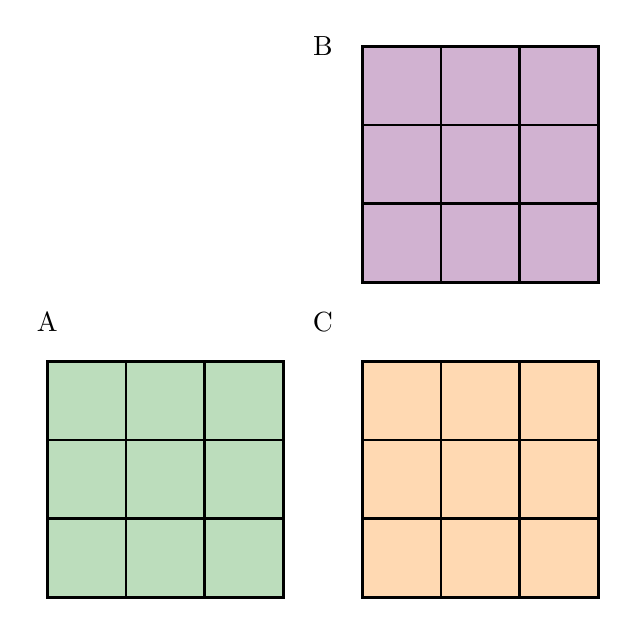
\begin{tikzpicture}
            % matrix A
            \node at (0, 3.5) {A};
            \fill[forestgreen!30] (0,2) rectangle (1,3);
            \draw[line width = 1pt] (0,2) rectangle (1,3);
            \fill[forestgreen!30] (0,1) rectangle (1,2);
            \draw[line width = 1pt] (0,1) rectangle (1,2);
            \fill[forestgreen!30] (0,0) rectangle (1,1);
            \draw[line width = 1pt] (0,0) rectangle (1,1);

            \fill[forestgreen!30] (1,2) rectangle (2,3);
            \draw[line width = 1pt] (1,2) rectangle (2,3);
            \fill[forestgreen!30] (1,1) rectangle (2,2);
            \draw[line width = 1pt] (1,1) rectangle (2,2);
            \fill[forestgreen!30] (1,0) rectangle (2,1);
            \draw[line width = 1pt] (1,0) rectangle (2,1);

            \fill[forestgreen!30] (2,2) rectangle (3,3);
            \draw[line width = 1pt] (2,2) rectangle (3,3);
            \fill[forestgreen!30] (2,1) rectangle (3,2);
            \draw[line width = 1pt] (2,1) rectangle (3,2);
            \fill[forestgreen!30] (2,0) rectangle (3,1);
            \draw[line width = 1pt] (2,0) rectangle (3,1);

            % matrix C
            \node at (3.5, 3.5) {C};
            \fill[orange!30] (4,0) rectangle (5,1);
            \draw[line width = 1pt] (4,0) rectangle (5,1);
            \fill[orange!30] (4,1) rectangle (5,2);
            \draw[line width = 1pt] (4,1) rectangle (5,2);
            \fill[orange!30] (4,2) rectangle (5,3);
            \draw[line width = 1pt] (4,2) rectangle (5,3);

            \fill[orange!30] (5,0) rectangle (6,1);
            \draw[line width = 1pt] (5,0) rectangle (6,1);
            \fill[orange!30] (5,1) rectangle (6,2);
            \draw[line width = 1pt] (5,1) rectangle (6,2);
            \fill[orange!30] (5,2) rectangle (6,3);
            \draw[line width = 1pt] (5,2) rectangle (6,3);

            \fill[orange!30] (6,0) rectangle (7,1);
            \draw[line width = 1pt] (6,0) rectangle (7,1);
            \fill[orange!30] (6,1) rectangle (7,2);
            \draw[line width = 1pt] (6,1) rectangle (7,2);
            \fill[orange!30] (6,2) rectangle (7,3);
            \draw[line width = 1pt] (6,2) rectangle (7,3);

            % Matrix B
            \node at (3.5, 7) {B};
            \fill[fancyViolet!30] (4,6) rectangle (5,7);
            \draw[line width = 1pt] (4,6) rectangle (5,7);
            \fill[fancyViolet!30] (4,5) rectangle (5,6);
            \draw[line width = 1pt] (4,5) rectangle (5,6);
            \fill[fancyViolet!30] (4,4) rectangle (5,5);
            \draw[line width = 1pt] (4,4) rectangle (5,5);

            \fill[fancyViolet!30] (5,6) rectangle (6,7);
            \draw[line width = 1pt] (5,6) rectangle (6,7);
            \fill[fancyViolet!30] (5,5) rectangle (6,6);
            \draw[line width = 1pt] (5,5) rectangle (6,6);
            \fill[fancyViolet!30] (5,4) rectangle (6,5);
            \draw[line width = 1pt] (5,4) rectangle (6,5);

            \fill[fancyViolet!30] (6,6) rectangle (7,7);
            \draw[line width = 1pt] (6,6) rectangle (7,7);
            \fill[fancyViolet!30] (6,5) rectangle (7,6);
            \draw[line width = 1pt] (6,5) rectangle (7,6);
            \fill[fancyViolet!30] (6,4) rectangle (7,5);
            \draw[line width = 1pt] (6,4) rectangle (7,5);

        \end{tikzpicture}
        \column{0.3\textwidth}
        \begin{math}
            C_{ij} = \sum_{k=0}^{K} A_{ik} B_{kj}
        \end{math}
    \end{columns}
\end{frame}

\begin{frame}{GEMM: example}
    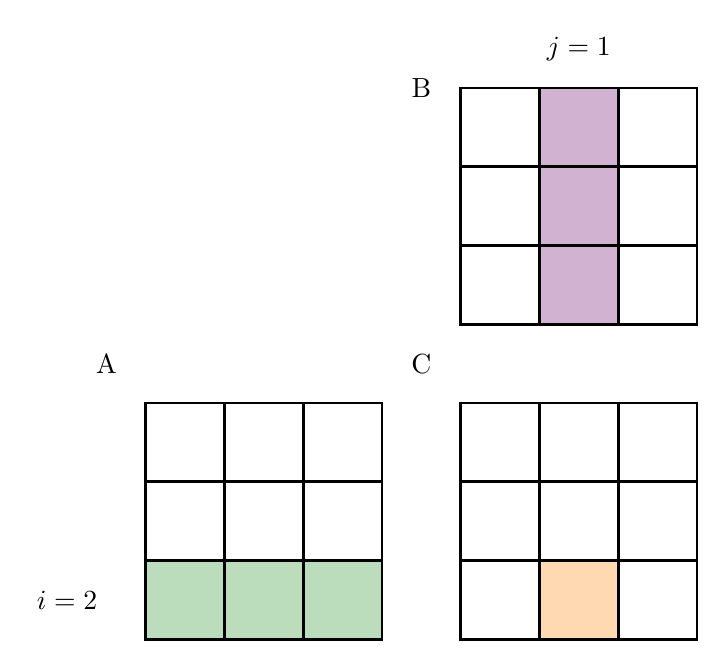
\begin{tikzpicture}
        % matrix A
        \node at (-1,0.5) {$i=2$};
        \node at (-0.5, 3.5) {A};
        %\fill[forestgreen!30] (0,2) rectangle (1,3);
        \draw[line width = 1pt] (0,2) rectangle (1,3);
        %\fill[forestgreen!30] (0,1) rectangle (1,2);
        \draw[line width = 1pt] (0,1) rectangle (1,2);
        \fill[forestgreen!30] (0,0) rectangle (1,1);
        \draw[line width = 1pt] (0,0) rectangle (1,1);

        %\fill[forestgreen!30] (1,2) rectangle (2,3);
        \draw[line width = 1pt] (1,2) rectangle (2,3);
        %\fill[forestgreen!30] (1,1) rectangle (2,2);
        \draw[line width = 1pt] (1,1) rectangle (2,2);
        \fill[forestgreen!30] (1,0) rectangle (2,1);
        \draw[line width = 1pt] (1,0) rectangle (2,1);

        %\fill[forestgreen!30] (2,2) rectangle (3,3);
        \draw[line width = 1pt] (2,2) rectangle (3,3);
        %\fill[forestgreen!30] (2,1) rectangle (3,2);
        \draw[line width = 1pt] (2,1) rectangle (3,2);
        \fill[forestgreen!30] (2,0) rectangle (3,1);
        \draw[line width = 1pt] (2,0) rectangle (3,1);

        % matrix C
        \node at (3.5, 3.5) {C};
        %\fill[orange!30] (4,0) rectangle (5,1);
        \draw[line width = 1pt] (4,0) rectangle (5,1);
        %\fill[orange!30] (4,1) rectangle (5,2);
        \draw[line width = 1pt] (4,1) rectangle (5,2);
        %\fill[orange!30] (4,2) rectangle (5,3);
        \draw[line width = 1pt] (4,2) rectangle (5,3);

        \fill[orange!30] (5,0) rectangle (6,1);
        \draw[line width = 1pt] (5,0) rectangle (6,1);
        %\fill[orange!30] (5,1) rectangle (6,2);
        \draw[line width = 1pt] (5,1) rectangle (6,2);
        %\fill[orange!30] (5,2) rectangle (6,3);
        \draw[line width = 1pt] (5,2) rectangle (6,3);

        %\fill[orange!30] (6,0) rectangle (7,1);
        \draw[line width = 1pt] (6,0) rectangle (7,1);
        %\fill[orange!30] (6,1) rectangle (7,2);
        \draw[line width = 1pt] (6,1) rectangle (7,2);
        %\fill[orange!30] (6,2) rectangle (7,3);
        \draw[line width = 1pt] (6,2) rectangle (7,3);

        % Matrix B
        \node at (5.5, 7.5) {$j=1$};
        \node at (3.5, 7) {B};
        %\fill[fancyViolet!30] (4,6) rectangle (5,7);
        \draw[line width = 1pt] (4,6) rectangle (5,7);
        %\fill[fancyViolet!30] (4,5) rectangle (5,6);
        \draw[line width = 1pt] (4,5) rectangle (5,6);
        %\fill[fancyViolet!30] (4,4) rectangle (5,5);
        \draw[line width = 1pt] (4,4) rectangle (5,5);

        \fill[fancyViolet!30] (5,6) rectangle (6,7);
        \draw[line width = 1pt] (5,6) rectangle (6,7);
        \fill[fancyViolet!30] (5,5) rectangle (6,6);
        \draw[line width = 1pt] (5,5) rectangle (6,6);
        \fill[fancyViolet!30] (5,4) rectangle (6,5);
        \draw[line width = 1pt] (5,4) rectangle (6,5);

        %\fill[fancyViolet!30] (6,6) rectangle (7,7);
        \draw[line width = 1pt] (6,6) rectangle (7,7);
        %\fill[fancyViolet!30] (6,5) rectangle (7,6);
        \draw[line width = 1pt] (6,5) rectangle (7,6);
        %\fill[fancyViolet!30] (6,4) rectangle (7,5);
        \draw[line width = 1pt] (6,4) rectangle (7,5);

    \end{tikzpicture}
\end{frame}

\begin{frame}{GEMM: example}
    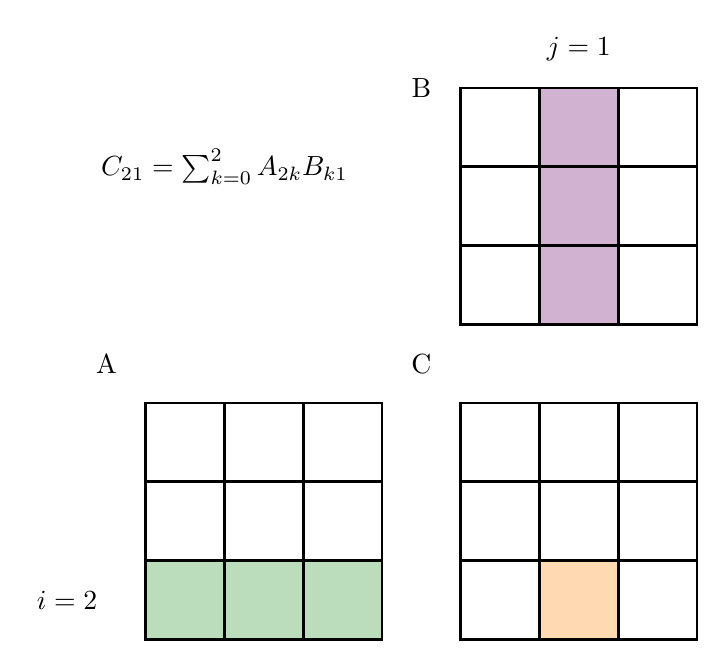
\begin{tikzpicture}
        %Formula
        \node at (1,6) {$C_{21} = \sum_{k=0}^{2} A_{2k} B_{k1}$};

        % matrix A
        \node at (-1,0.5) {$i=2$};
        \node at (-0.5, 3.5) {A};
        %\fill[forestgreen!30] (0,2) rectangle (1,3);
        \draw[line width = 1pt] (0,2) rectangle (1,3);
        %\fill[forestgreen!30] (0,1) rectangle (1,2);
        \draw[line width = 1pt] (0,1) rectangle (1,2);
        \fill[forestgreen!30] (0,0) rectangle (1,1);
        \draw[line width = 1pt] (0,0) rectangle (1,1);

        %\fill[forestgreen!30] (1,2) rectangle (2,3);
        \draw[line width = 1pt] (1,2) rectangle (2,3);
        %\fill[forestgreen!30] (1,1) rectangle (2,2);
        \draw[line width = 1pt] (1,1) rectangle (2,2);
        \fill[forestgreen!30] (1,0) rectangle (2,1);
        \draw[line width = 1pt] (1,0) rectangle (2,1);

        %\fill[forestgreen!30] (2,2) rectangle (3,3);
        \draw[line width = 1pt] (2,2) rectangle (3,3);
        %\fill[forestgreen!30] (2,1) rectangle (3,2);
        \draw[line width = 1pt] (2,1) rectangle (3,2);
        \fill[forestgreen!30] (2,0) rectangle (3,1);
        \draw[line width = 1pt] (2,0) rectangle (3,1);

        % matrix C
        \node at (3.5, 3.5) {C};
        %\fill[orange!30] (4,0) rectangle (5,1);
        \draw[line width = 1pt] (4,0) rectangle (5,1);
        %\fill[orange!30] (4,1) rectangle (5,2);
        \draw[line width = 1pt] (4,1) rectangle (5,2);
        %\fill[orange!30] (4,2) rectangle (5,3);
        \draw[line width = 1pt] (4,2) rectangle (5,3);

        \fill[orange!30] (5,0) rectangle (6,1);
        \draw[line width = 1pt] (5,0) rectangle (6,1);
        %\fill[orange!30] (5,1) rectangle (6,2);
        \draw[line width = 1pt] (5,1) rectangle (6,2);
        %\fill[orange!30] (5,2) rectangle (6,3);
        \draw[line width = 1pt] (5,2) rectangle (6,3);

        %\fill[orange!30] (6,0) rectangle (7,1);
        \draw[line width = 1pt] (6,0) rectangle (7,1);
        %\fill[orange!30] (6,1) rectangle (7,2);
        \draw[line width = 1pt] (6,1) rectangle (7,2);
        %\fill[orange!30] (6,2) rectangle (7,3);
        \draw[line width = 1pt] (6,2) rectangle (7,3);

        % Matrix B
        \node at (5.5, 7.5) {$j=1$};
        \node at (3.5, 7) {B};
        %\fill[fancyViolet!30] (4,6) rectangle (5,7);
        \draw[line width = 1pt] (4,6) rectangle (5,7);
        %\fill[fancyViolet!30] (4,5) rectangle (5,6);
        \draw[line width = 1pt] (4,5) rectangle (5,6);
        %\fill[fancyViolet!30] (4,4) rectangle (5,5);
        \draw[line width = 1pt] (4,4) rectangle (5,5);

        \fill[fancyViolet!30] (5,6) rectangle (6,7);
        \draw[line width = 1pt] (5,6) rectangle (6,7);
        \fill[fancyViolet!30] (5,5) rectangle (6,6);
        \draw[line width = 1pt] (5,5) rectangle (6,6);
        \fill[fancyViolet!30] (5,4) rectangle (6,5);
        \draw[line width = 1pt] (5,4) rectangle (6,5);

        %\fill[fancyViolet!30] (6,6) rectangle (7,7);
        \draw[line width = 1pt] (6,6) rectangle (7,7);
        %\fill[fancyViolet!30] (6,5) rectangle (7,6);
        \draw[line width = 1pt] (6,5) rectangle (7,6);
        %\fill[fancyViolet!30] (6,4) rectangle (7,5);
        \draw[line width = 1pt] (6,4) rectangle (7,5);

    \end{tikzpicture}
\end{frame}

\begin{frame}{GEMM: example}
    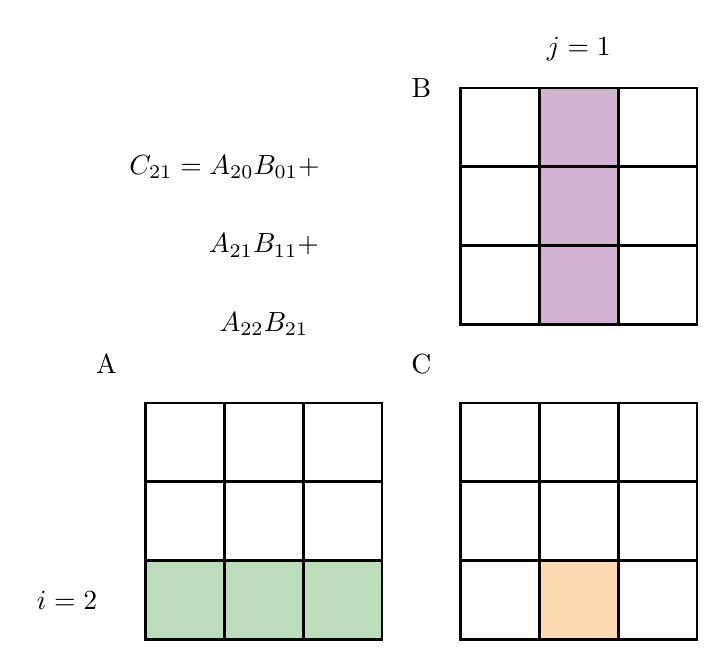
\begin{tikzpicture}
        %Formula
        \node at (1,6) {$C_{21} = A_{20}B_{01} + $};
        \node at (1.5,5) {$A_{21}B_{11} +$};
        \node at (1.5,4) {$A_{22}B_{21}$};
        % matrix A
        \node at (-1,0.5) {$i=2$};
        \node at (-0.5, 3.5) {A};
        %\fill[forestgreen!30] (0,2) rectangle (1,3);
        \draw[line width = 1pt] (0,2) rectangle (1,3);
        %\fill[forestgreen!30] (0,1) rectangle (1,2);
        \draw[line width = 1pt] (0,1) rectangle (1,2);
        \fill[forestgreen!30] (0,0) rectangle (1,1);
        \draw[line width = 1pt] (0,0) rectangle (1,1);

        %\fill[forestgreen!30] (1,2) rectangle (2,3);
        \draw[line width = 1pt] (1,2) rectangle (2,3);
        %\fill[forestgreen!30] (1,1) rectangle (2,2);
        \draw[line width = 1pt] (1,1) rectangle (2,2);
        \fill[forestgreen!30] (1,0) rectangle (2,1);
        \draw[line width = 1pt] (1,0) rectangle (2,1);

        %\fill[forestgreen!30] (2,2) rectangle (3,3);
        \draw[line width = 1pt] (2,2) rectangle (3,3);
        %\fill[forestgreen!30] (2,1) rectangle (3,2);
        \draw[line width = 1pt] (2,1) rectangle (3,2);
        \fill[forestgreen!30] (2,0) rectangle (3,1);
        \draw[line width = 1pt] (2,0) rectangle (3,1);

        % matrix C
        \node at (3.5, 3.5) {C};
        %\fill[orange!30] (4,0) rectangle (5,1);
        \draw[line width = 1pt] (4,0) rectangle (5,1);
        %\fill[orange!30] (4,1) rectangle (5,2);
        \draw[line width = 1pt] (4,1) rectangle (5,2);
        %\fill[orange!30] (4,2) rectangle (5,3);
        \draw[line width = 1pt] (4,2) rectangle (5,3);

        \fill[orange!30] (5,0) rectangle (6,1);
        \draw[line width = 1pt] (5,0) rectangle (6,1);
        %\fill[orange!30] (5,1) rectangle (6,2);
        \draw[line width = 1pt] (5,1) rectangle (6,2);
        %\fill[orange!30] (5,2) rectangle (6,3);
        \draw[line width = 1pt] (5,2) rectangle (6,3);

        %\fill[orange!30] (6,0) rectangle (7,1);
        \draw[line width = 1pt] (6,0) rectangle (7,1);
        %\fill[orange!30] (6,1) rectangle (7,2);
        \draw[line width = 1pt] (6,1) rectangle (7,2);
        %\fill[orange!30] (6,2) rectangle (7,3);
        \draw[line width = 1pt] (6,2) rectangle (7,3);

        % Matrix B
        \node at (5.5, 7.5) {$j=1$};
        \node at (3.5, 7) {B};
        %\fill[fancyViolet!30] (4,6) rectangle (5,7);
        \draw[line width = 1pt] (4,6) rectangle (5,7);
        %\fill[fancyViolet!30] (4,5) rectangle (5,6);
        \draw[line width = 1pt] (4,5) rectangle (5,6);
        %\fill[fancyViolet!30] (4,4) rectangle (5,5);
        \draw[line width = 1pt] (4,4) rectangle (5,5);

        \fill[fancyViolet!30] (5,6) rectangle (6,7);
        \draw[line width = 1pt] (5,6) rectangle (6,7);
        \fill[fancyViolet!30] (5,5) rectangle (6,6);
        \draw[line width = 1pt] (5,5) rectangle (6,6);
        \fill[fancyViolet!30] (5,4) rectangle (6,5);
        \draw[line width = 1pt] (5,4) rectangle (6,5);

        %\fill[fancyViolet!30] (6,6) rectangle (7,7);
        \draw[line width = 1pt] (6,6) rectangle (7,7);
        %\fill[fancyViolet!30] (6,5) rectangle (7,6);
        \draw[line width = 1pt] (6,5) rectangle (7,6);
        %\fill[fancyViolet!30] (6,4) rectangle (7,5);
        \draw[line width = 1pt] (6,4) rectangle (7,5);

    \end{tikzpicture}
\end{frame}

\begin{frame}{Map Reduce and STF}
    \begin{columns}
        \column{0.6\textwidth}
        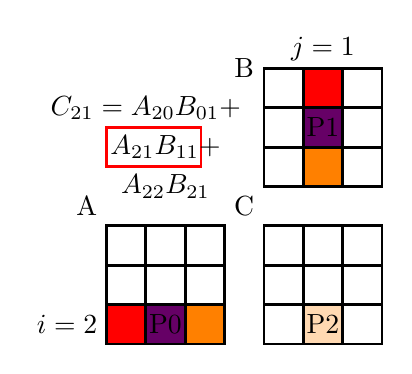
\begin{tikzpicture}[scale=0.5]

            \node at (1,6) {$C_{21} = A_{20}B_{01} + $};
            \draw[red, line width = 1pt] (0,5.5) rectangle (2.4,4.5);
            \node at (1.5,5) {$A_{21}B_{11} +$};
            \node at (1.5,4) {$A_{22}B_{21}$};
            % matrix A
            \node at (-1,0.5) {$i=2$};
            \node at (-0.5, 3.5) {A};
            \draw[line width = 1pt] (0,2) rectangle (1,3);
            \draw[line width = 1pt] (0,1) rectangle (1,2);
            \fill[red] (0,0) rectangle (1,1);
            \draw[line width = 1pt] (0,0) rectangle (1,1);

            \draw[line width = 1pt] (1,2) rectangle (2,3);
            \draw[line width = 1pt] (1,1) rectangle (2,2);
            \fill[fancyViolet] (1,0) rectangle (2,1);
            \node at (1.5,0.5) {P0};
            \draw[line width = 1pt] (1,0) rectangle (2,1);

            \draw[line width = 1pt] (2,2) rectangle (3,3);
            \draw[line width = 1pt] (2,1) rectangle (3,2);
            \fill[orange] (2,0) rectangle (3,1);
            \draw[line width = 1pt] (2,0) rectangle (3,1);

            % matrix C
            \node at (3.5, 3.5) {C};
            \draw[line width = 1pt] (4,0) rectangle (5,1);
            \draw[line width = 1pt] (4,1) rectangle (5,2);
            \draw[line width = 1pt] (4,2) rectangle (5,3);

            \fill[orange!30] (5,0) rectangle (6,1);
            \draw[line width = 1pt] (5,0) rectangle (6,1);
            \node at (5.5,0.5) {P2};
            \draw[line width = 1pt] (5,1) rectangle (6,2);
            \draw[line width = 1pt] (5,2) rectangle (6,3);

            \draw[line width = 1pt] (6,0) rectangle (7,1);
            \draw[line width = 1pt] (6,1) rectangle (7,2);
            \draw[line width = 1pt] (6,2) rectangle (7,3);

            % Matrix B
            \node at (5.5, 7.5) {$j=1$};
            \node at (3.5, 7) {B};
            \draw[line width = 1pt] (4,6) rectangle (5,7);
            \draw[line width = 1pt] (4,5) rectangle (5,6);
            \draw[line width = 1pt] (4,4) rectangle (5,5);

            \fill[red] (5,6) rectangle (6,7);
            \draw[line width = 1pt] (5,6) rectangle (6,7);
            \fill[fancyViolet] (5,5) rectangle (6,6);
            \node at (5.5,5.5) {P1};
            \draw[line width = 1pt] (5,5) rectangle (6,6);
            \fill[orange] (5,4) rectangle (6,5);
            \draw[line width = 1pt] (5,4) rectangle (6,5);

            \draw[line width = 1pt] (6,6) rectangle (7,7);
            \draw[line width = 1pt] (6,5) rectangle (7,6);
            \draw[line width = 1pt] (6,4) rectangle (7,5);

        \end{tikzpicture}

        % Datamap sample:
        % \begin{tikzpicture}[scale=0.5]
        %     \node at (0,4.5) { };
        %     \draw[line width = 1pt] (0,0) rectangle (1,1);
        %     \node at (0.5,0.5) {P1};
        %     \draw[line width = 1pt] (0,1) rectangle (1,2);
        %     \node at (0.5,1.5) {P2};
        %     \draw[line width = 1pt] (0,2) rectangle (1,3);
        %     \node at (0.5,2.5) {P2};

        %     \draw[line width = 1pt] (1,0) rectangle (2,1);
        %     \node at (1.5,0.5) {P1};
        %     \draw[line width = 1pt] (1,1) rectangle (2,2);
        %     \node at (1.5,1.5) {P3};
        %     \draw[line width = 1pt] (1,2) rectangle (2,3);
        %     \node at (1.5,2.5) {P0};

        %     \draw[line width = 1pt] (2,0) rectangle (3,1);
        %     \node at (2.5,0.5) {P0};
        %     \draw[line width = 1pt] (2,1) rectangle (3,2);
        %     \node at (2.5,1.5) {P3};
        %     \draw[line width = 1pt] (2,2) rectangle (3,3);
        %     \node at (2.5,2.5) {P2};
        % \end{tikzpicture}

        \column{0.45\textwidth}
            \begin{block}{Map Reduce (MR)}
                \begin{itemize}
                    \item \color{red} gemm($C_{211}$, $A_{20}$, $B_{01}$)
                    \item \color{fancyViolet} gemm($C_{212}$, $A_{21}$, $B_{11}$)
                    \item \color{orange} gemm($C_{213}$, $A_{22}$, $B_{21}$)
                    \item \color{black} After all : \\ Reduce($C_{211}$, $C_{212}$, $C_{213}$)
                \end{itemize}
            \end{block}
            \begin{exampleblock}{Single task flow (STF)}
                \begin{enumerate}
                    \item \color{red} gemm($C_{21}$, $A_{20}$, $B_{01}$)
                    \item \color{fancyViolet} gemm($C_{21}$, $A_{21}$, $B_{11}$)
                    \item \color{orange} gemm($C_{21}$, $A_{22}$, $B_{21}$)
                \end{enumerate}
            \end{exampleblock}
    \end{columns}
    
\end{frame}

\begin{frame}[t]{Execution model : MPI}
    \begin{columns}
        \column{0.6\textwidth}
        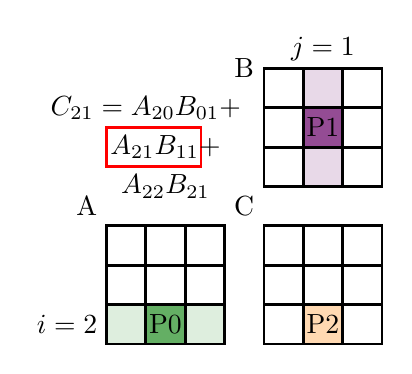
\begin{tikzpicture}[scale=0.5]

            \node at (1,6) {$C_{21} = A_{20}B_{01} + $};
            \draw[red, line width = 1pt] (0,5.5) rectangle (2.4,4.5);
            \node at (1.5,5) {$A_{21}B_{11} +$};
            \node at (1.5,4) {$A_{22}B_{21}$};
            % matrix A
            \node at (-1,0.5) {$i=2$};
            \node at (-0.5, 3.5) {A};
            \draw[line width = 1pt] (0,2) rectangle (1,3);
            \draw[line width = 1pt] (0,1) rectangle (1,2);
            \fill[forestgreen!15] (0,0) rectangle (1,1);
            \draw[line width = 1pt] (0,0) rectangle (1,1);

            \draw[line width = 1pt] (1,2) rectangle (2,3);
            \draw[line width = 1pt] (1,1) rectangle (2,2);
            \fill[forestgreen!70] (1,0) rectangle (2,1);
            \node at (1.5,0.5) {P0};
            \draw[line width = 1pt] (1,0) rectangle (2,1);

            \draw[line width = 1pt] (2,2) rectangle (3,3);
            \draw[line width = 1pt] (2,1) rectangle (3,2);
            \fill[forestgreen!15] (2,0) rectangle (3,1);
            \draw[line width = 1pt] (2,0) rectangle (3,1);

            % matrix C
            \node at (3.5, 3.5) {C};
            \draw[line width = 1pt] (4,0) rectangle (5,1);
            \draw[line width = 1pt] (4,1) rectangle (5,2);
            \draw[line width = 1pt] (4,2) rectangle (5,3);

            \fill[orange!30] (5,0) rectangle (6,1);
            \draw[line width = 1pt] (5,0) rectangle (6,1);
            \node at (5.5,0.5) {P2};
            \draw[line width = 1pt] (5,1) rectangle (6,2);
            \draw[line width = 1pt] (5,2) rectangle (6,3);

            \draw[line width = 1pt] (6,0) rectangle (7,1);
            \draw[line width = 1pt] (6,1) rectangle (7,2);
            \draw[line width = 1pt] (6,2) rectangle (7,3);

            % Matrix B
            \node at (5.5, 7.5) {$j=1$};
            \node at (3.5, 7) {B};
            \draw[line width = 1pt] (4,6) rectangle (5,7);
            \draw[line width = 1pt] (4,5) rectangle (5,6);
            \draw[line width = 1pt] (4,4) rectangle (5,5);

            \fill[fancyViolet!15] (5,6) rectangle (6,7);
            \draw[line width = 1pt] (5,6) rectangle (6,7);
            \fill[fancyViolet!70] (5,5) rectangle (6,6);
            \node at (5.5,5.5) {P1};
            \draw[line width = 1pt] (5,5) rectangle (6,6);
            \fill[fancyViolet!15] (5,4) rectangle (6,5);
            \draw[line width = 1pt] (5,4) rectangle (6,5);

            \draw[line width = 1pt] (6,6) rectangle (7,7);
            \draw[line width = 1pt] (6,5) rectangle (7,6);
            \draw[line width = 1pt] (6,4) rectangle (7,5);

        \end{tikzpicture}

        \begin{columns}
            \column{0.4\textwidth}
            \begin{equation*}
                \begin{aligned}
                    P1 \,  & \underrightarrow{B} \, P2 \\
                    P0 \,& \underrightarrow{A} \,P2 \\
                    P2 \,& \underleftarrow{A}  \,P0  \\
                    P2 \,& \underleftarrow{B}  \,P1 \\
                    P2 \,& GEMM(A,B,C)
                \end{aligned}
            \end{equation*}
            \column{0.4\textwidth}
            \begin{align*}
                \rightarrow : & isend\ block \\
                \leftarrow :  & recv\ block
            \end{align*}
        \end{columns}

        \column{0.4\textwidth}
            \begin{block}{Programation model (MR)}
                \begin{itemize}
                    \item Target : Distributed memory
                    \item Dependency : Explicit    
                \end{itemize}
            \end{block}
            \begin{exampleblock}{Execution model}
                \begin{itemize}
                    \item Control : Distributed flow
                    \item Execution : "In Order (IO)"
                \end{itemize}
            \end{exampleblock}
    \end{columns}
\end{frame}

\begin{frame}[t]{Execution model : OpenMP tasks}
    \begin{columns}
        \column{0.6\textwidth}
        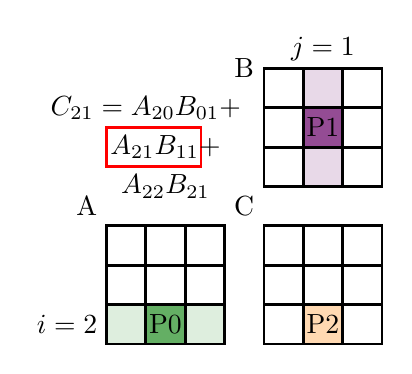
\begin{tikzpicture}[scale=0.5]

            \node at (1,6) {$C_{21} = A_{20}B_{01} + $};
            \draw[red, line width = 1pt] (0,5.5) rectangle (2.4,4.5);
            \node at (1.5,5) {$A_{21}B_{11} +$};
            \node at (1.5,4) {$A_{22}B_{21}$};
            % matrix A
            \node at (-1,0.5) {$i=2$};
            \node at (-0.5, 3.5) {A};
            \draw[line width = 1pt] (0,2) rectangle (1,3);
            \draw[line width = 1pt] (0,1) rectangle (1,2);
            \fill[forestgreen!15] (0,0) rectangle (1,1);
            \draw[line width = 1pt] (0,0) rectangle (1,1);

            \draw[line width = 1pt] (1,2) rectangle (2,3);
            \draw[line width = 1pt] (1,1) rectangle (2,2);
            \fill[forestgreen!70] (1,0) rectangle (2,1);
            \node at (1.5,0.5) {P0};
            \draw[line width = 1pt] (1,0) rectangle (2,1);

            \draw[line width = 1pt] (2,2) rectangle (3,3);
            \draw[line width = 1pt] (2,1) rectangle (3,2);
            \fill[forestgreen!15] (2,0) rectangle (3,1);
            \draw[line width = 1pt] (2,0) rectangle (3,1);

            % matrix C
            \node at (3.5, 3.5) {C};
            \draw[line width = 1pt] (4,0) rectangle (5,1);
            \draw[line width = 1pt] (4,1) rectangle (5,2);
            \draw[line width = 1pt] (4,2) rectangle (5,3);

            \fill[orange!30] (5,0) rectangle (6,1);
            \draw[line width = 1pt] (5,0) rectangle (6,1);
            \node at (5.5,0.5) {P2};
            \draw[line width = 1pt] (5,1) rectangle (6,2);
            \draw[line width = 1pt] (5,2) rectangle (6,3);

            \draw[line width = 1pt] (6,0) rectangle (7,1);
            \draw[line width = 1pt] (6,1) rectangle (7,2);
            \draw[line width = 1pt] (6,2) rectangle (7,3);

            % Matrix B
            \node at (5.5, 7.5) {$j=1$};
            \node at (3.5, 7) {B};
            \draw[line width = 1pt] (4,6) rectangle (5,7);
            \draw[line width = 1pt] (4,5) rectangle (5,6);
            \draw[line width = 1pt] (4,4) rectangle (5,5);

            \fill[fancyViolet!15] (5,6) rectangle (6,7);
            \draw[line width = 1pt] (5,6) rectangle (6,7);
            \fill[fancyViolet!70] (5,5) rectangle (6,6);
            \node at (5.5,5.5) {P1};
            \draw[line width = 1pt] (5,5) rectangle (6,6);
            \fill[fancyViolet!15] (5,4) rectangle (6,5);
            \draw[line width = 1pt] (5,4) rectangle (6,5);

            \draw[line width = 1pt] (6,6) rectangle (7,7);
            \draw[line width = 1pt] (6,5) rectangle (7,6);
            \draw[line width = 1pt] (6,4) rectangle (7,5);

        \end{tikzpicture}
        \phantom{T} \\
        \phantom{T} \\
        Tasks :
        \begin{itemize}
            \item $GEMM(A_{2k}:R, B_{k1}:R, C_{21}:W) $
        \end{itemize}

        R : Read access \\
        W : Write access

        \column{0.4\textwidth}
        \begin{block}{Programation model (STF)}
            \begin{itemize}
                \item Target : Multicore architecture / Unified memory
                \item Dependency : Implicit (Data hazard)
            \end{itemize}
        \end{block}
        \begin{exampleblock}{Execution model}
            \begin{itemize}
                \item Control : Master / slave
                \item Execution : "Out Of Order (OOO)"
            \end{itemize}
        \end{exampleblock}
    \end{columns}
\end{frame}

\begin{frame}[t]{Execution model : MPI with tasks}
    \begin{columns}
        \column{0.6\textwidth}

        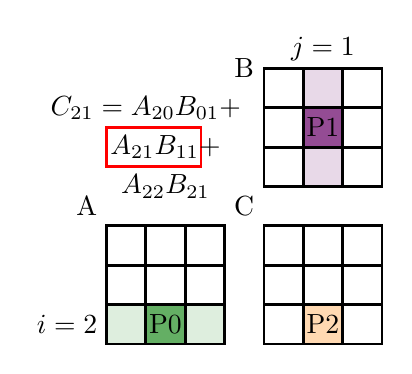
\begin{tikzpicture}[scale=0.5]

            \node at (1,6) {$C_{21} = A_{20}B_{01} + $};
            \draw[red, line width = 1pt] (0,5.5) rectangle (2.4,4.5);
            \node at (1.5,5) {$A_{21}B_{11} +$};
            \node at (1.5,4) {$A_{22}B_{21}$};
            % matrix A
            \node at (-1,0.5) {$i=2$};
            \node at (-0.5, 3.5) {A};
            \draw[line width = 1pt] (0,2) rectangle (1,3);
            \draw[line width = 1pt] (0,1) rectangle (1,2);
            \fill[forestgreen!15] (0,0) rectangle (1,1);
            \draw[line width = 1pt] (0,0) rectangle (1,1);

            \draw[line width = 1pt] (1,2) rectangle (2,3);
            \draw[line width = 1pt] (1,1) rectangle (2,2);
            \fill[forestgreen!70] (1,0) rectangle (2,1);
            \node at (1.5,0.5) {P0};
            \draw[line width = 1pt] (1,0) rectangle (2,1);

            \draw[line width = 1pt] (2,2) rectangle (3,3);
            \draw[line width = 1pt] (2,1) rectangle (3,2);
            \fill[forestgreen!15] (2,0) rectangle (3,1);
            \draw[line width = 1pt] (2,0) rectangle (3,1);

            % matrix C
            \node at (3.5, 3.5) {C};
            \draw[line width = 1pt] (4,0) rectangle (5,1);
            \draw[line width = 1pt] (4,1) rectangle (5,2);
            \draw[line width = 1pt] (4,2) rectangle (5,3);

            \fill[orange!30] (5,0) rectangle (6,1);
            \draw[line width = 1pt] (5,0) rectangle (6,1);
            \node at (5.5,0.5) {P2};
            \draw[line width = 1pt] (5,1) rectangle (6,2);
            \draw[line width = 1pt] (5,2) rectangle (6,3);

            \draw[line width = 1pt] (6,0) rectangle (7,1);
            \draw[line width = 1pt] (6,1) rectangle (7,2);
            \draw[line width = 1pt] (6,2) rectangle (7,3);

            % Matrix B
            \node at (5.5, 7.5) {$j=1$};
            \node at (3.5, 7) {B};
            \draw[line width = 1pt] (4,6) rectangle (5,7);
            \draw[line width = 1pt] (4,5) rectangle (5,6);
            \draw[line width = 1pt] (4,4) rectangle (5,5);

            \fill[fancyViolet!15] (5,6) rectangle (6,7);
            \draw[line width = 1pt] (5,6) rectangle (6,7);
            \fill[fancyViolet!70] (5,5) rectangle (6,6);
            \node at (5.5,5.5) {P1};
            \draw[line width = 1pt] (5,5) rectangle (6,6);
            \fill[fancyViolet!15] (5,4) rectangle (6,5);
            \draw[line width = 1pt] (5,4) rectangle (6,5);

            \draw[line width = 1pt] (6,6) rectangle (7,7);
            \draw[line width = 1pt] (6,5) rectangle (7,6);
            \draw[line width = 1pt] (6,4) rectangle (7,5);

        \end{tikzpicture}
        \begin{columns}
            \column{0.4\textwidth}
            \begin{equation*}
                \begin{aligned}
                    P1 \,  & \underrightarrow{B} \, P2 \\
                    P0 \,& \underrightarrow{A} \,P2 \\
                    P2 \,& \underleftarrow{A}  \,P0  \\
                    P2 \,& \underleftarrow{B}  \,P1 \\
                    P2 \,& GEMM(A,B,C)
                \end{aligned}
            \end{equation*}
            \column{0.4\textwidth}
            \begin{align*}
                \rightarrow\ : & task\ isend\ block \\
                \leftarrow\ :  & task\ recv\ block \\
                GEMM : & task\ GEMM
            \end{align*}
        \end{columns}

        \column{0.4\textwidth}
        \begin{block}{Programation model (MR/STF)}
            \begin{itemize}
                \item Target : Distributed memory
                \item Dependency : Explicit
            \end{itemize}
        \end{block}
        \begin{exampleblock}{Execution model}
            \begin{itemize}
                \item Control : Master/Slave on node and distributed flow between nodes
                \item Execution : "In Order (IO)"
            \end{itemize}
        \end{exampleblock}
    \end{columns}
\end{frame}

\begin{frame}[fragile, t]{Execution model : Chameleon}
    \begin{columns}
        \column{0.6\textwidth}
        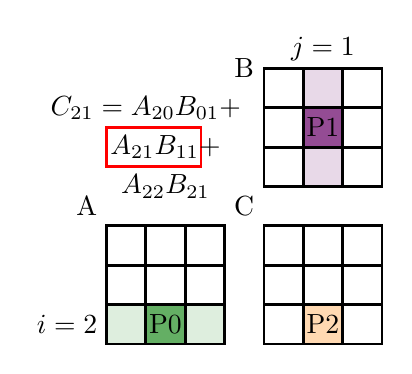
\begin{tikzpicture}[scale=0.5]

            \node at (1,6) {$C_{21} = A_{20}B_{01} + $};
            \draw[red, line width = 1pt] (0,5.5) rectangle (2.4,4.5);
            \node at (1.5,5) {$A_{21}B_{11} +$};
            \node at (1.5,4) {$A_{22}B_{21}$};
            % matrix A
            \node at (-1,0.5) {$i=2$};
            \node at (-0.5, 3.5) {A};
            \draw[line width = 1pt] (0,2) rectangle (1,3);
            \draw[line width = 1pt] (0,1) rectangle (1,2);
            \fill[forestgreen!15] (0,0) rectangle (1,1);
            \draw[line width = 1pt] (0,0) rectangle (1,1);

            \draw[line width = 1pt] (1,2) rectangle (2,3);
            \draw[line width = 1pt] (1,1) rectangle (2,2);
            \fill[forestgreen!70] (1,0) rectangle (2,1);
            \node at (1.5,0.5) {P0};
            \draw[line width = 1pt] (1,0) rectangle (2,1);

            \draw[line width = 1pt] (2,2) rectangle (3,3);
            \draw[line width = 1pt] (2,1) rectangle (3,2);
            \fill[forestgreen!15] (2,0) rectangle (3,1);
            \draw[line width = 1pt] (2,0) rectangle (3,1);

            % matrix C
            \node at (3.5, 3.5) {C};
            \draw[line width = 1pt] (4,0) rectangle (5,1);
            \draw[line width = 1pt] (4,1) rectangle (5,2);
            \draw[line width = 1pt] (4,2) rectangle (5,3);

            \fill[orange!30] (5,0) rectangle (6,1);
            \draw[line width = 1pt] (5,0) rectangle (6,1);
            \node at (5.5,0.5) {P2};
            \draw[line width = 1pt] (5,1) rectangle (6,2);
            \draw[line width = 1pt] (5,2) rectangle (6,3);

            \draw[line width = 1pt] (6,0) rectangle (7,1);
            \draw[line width = 1pt] (6,1) rectangle (7,2);
            \draw[line width = 1pt] (6,2) rectangle (7,3);

            % Matrix B
            \node at (5.5, 7.5) {$j=1$};
            \node at (3.5, 7) {B};
            \draw[line width = 1pt] (4,6) rectangle (5,7);
            \draw[line width = 1pt] (4,5) rectangle (5,6);
            \draw[line width = 1pt] (4,4) rectangle (5,5);

            \fill[fancyViolet!15] (5,6) rectangle (6,7);
            \draw[line width = 1pt] (5,6) rectangle (6,7);
            \fill[fancyViolet!70] (5,5) rectangle (6,6);
            \node at (5.5,5.5) {P1};
            \draw[line width = 1pt] (5,5) rectangle (6,6);
            \fill[fancyViolet!15] (5,4) rectangle (6,5);
            \draw[line width = 1pt] (5,4) rectangle (6,5);

            \draw[line width = 1pt] (6,6) rectangle (7,7);
            \draw[line width = 1pt] (6,5) rectangle (7,6);
            \draw[line width = 1pt] (6,4) rectangle (7,5);

        \end{tikzpicture}

            \begin{lstlisting}
Forall i:
    Forall j:
        Forall k:
            GEMM(Aik, Bkj, Cij)
            \end{lstlisting}

        \column{0.4\textwidth}
        \begin{block}{Programation model (STF)}
            \begin{itemize}
                \item Target : Multinode
                \item Dependency : Implicit
            \end{itemize}
        \end{block}
        \begin{exampleblock}{Execution model}
            \begin{itemize}
                \item Control : Master/Slave on node and distributed flow between nodes
                \item Execution : "Out Of Order (OOO)"
            \end{itemize}
        \end{exampleblock}
    \end{columns}
\end{frame}

\begin{frame}{Preliminary result}
    \begin{columns}
        \column{0.48\textwidth}
        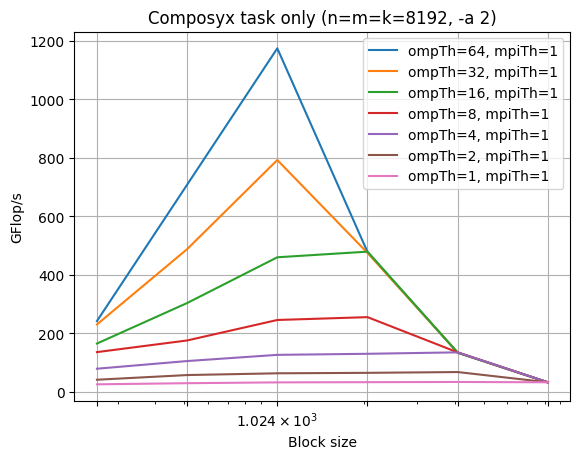
\includegraphics[width=\textwidth]{images/composyx_task.png}
        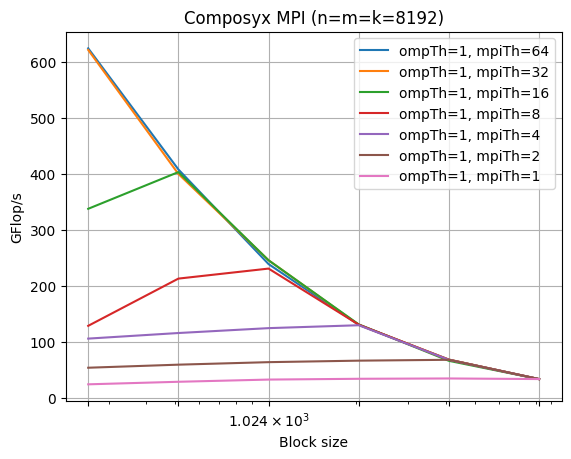
\includegraphics[width=\textwidth]{images/composyx_MPI.png}
        \column{0.48\textwidth}
        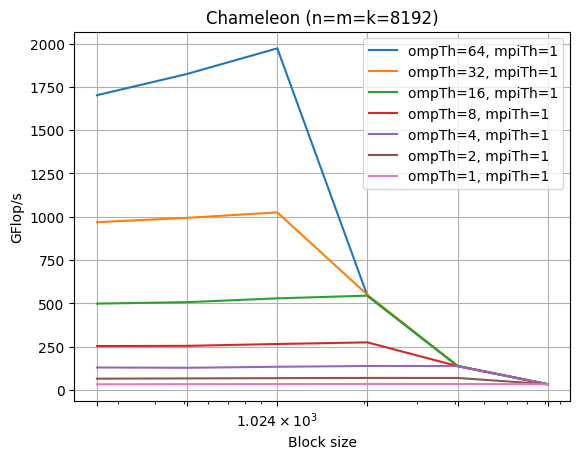
\includegraphics[width=\textwidth]{images/chameleon_bench.png}
        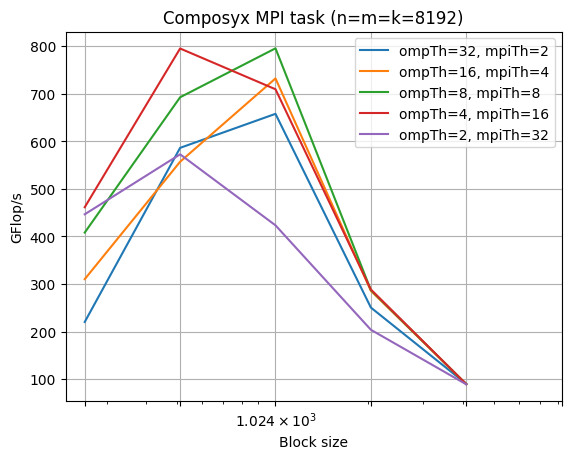
\includegraphics[width=\textwidth]{images/composix_hybrid.png}
        
    \end{columns}
\end{frame}

\begin{frame}{Algorithm Variation}
    \begin{columns}
    \column{0.6\textwidth}
    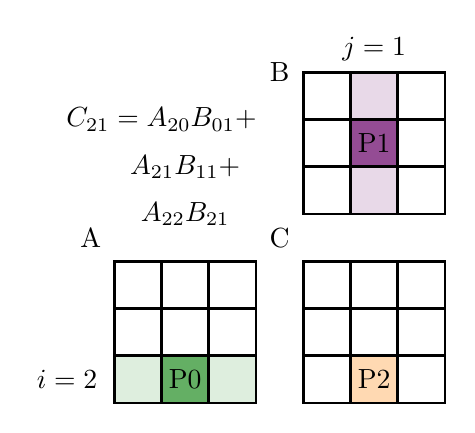
\begin{tikzpicture}[scale=0.6]

        \node at (1,6) {$C_{21} = A_{20}B_{01} + $};
        %\draw[red, line width = 1pt] (0,5.5) rectangle (2.4,4.5);
        \node at (1.5,5) {$A_{21}B_{11} +$};
        \node at (1.5,4) {$A_{22}B_{21}$};
        % matrix A
        \node at (-1,0.5) {$i=2$};
        \node at (-0.5, 3.5) {A};
        \draw[line width = 1pt] (0,2) rectangle (1,3);
        \draw[line width = 1pt] (0,1) rectangle (1,2);
        \fill[forestgreen!15] (0,0) rectangle (1,1);
        \draw[line width = 1pt] (0,0) rectangle (1,1);

        \draw[line width = 1pt] (1,2) rectangle (2,3);
        \draw[line width = 1pt] (1,1) rectangle (2,2);
        \fill[forestgreen!70] (1,0) rectangle (2,1);
        \node at (1.5,0.5) {P0};
        \draw[line width = 1pt] (1,0) rectangle (2,1);

        \draw[line width = 1pt] (2,2) rectangle (3,3);
        \draw[line width = 1pt] (2,1) rectangle (3,2);
        \fill[forestgreen!15] (2,0) rectangle (3,1);
        \draw[line width = 1pt] (2,0) rectangle (3,1);

        % matrix C
        \node at (3.5, 3.5) {C};
        \draw[line width = 1pt] (4,0) rectangle (5,1);
        \draw[line width = 1pt] (4,1) rectangle (5,2);
        \draw[line width = 1pt] (4,2) rectangle (5,3);

        \fill[orange!30] (5,0) rectangle (6,1);
        \draw[line width = 1pt] (5,0) rectangle (6,1);
        \node at (5.5,0.5) {P2};
        \draw[line width = 1pt] (5,1) rectangle (6,2);
        \draw[line width = 1pt] (5,2) rectangle (6,3);

        \draw[line width = 1pt] (6,0) rectangle (7,1);
        \draw[line width = 1pt] (6,1) rectangle (7,2);
        \draw[line width = 1pt] (6,2) rectangle (7,3);

        % Matrix B
        \node at (5.5, 7.5) {$j=1$};
        \node at (3.5, 7) {B};
        \draw[line width = 1pt] (4,6) rectangle (5,7);
        \draw[line width = 1pt] (4,5) rectangle (5,6);
        \draw[line width = 1pt] (4,4) rectangle (5,5);

        \fill[fancyViolet!15] (5,6) rectangle (6,7);
        \draw[line width = 1pt] (5,6) rectangle (6,7);
        \fill[fancyViolet!70] (5,5) rectangle (6,6);
        \node at (5.5,5.5) {P1};
        \draw[line width = 1pt] (5,5) rectangle (6,6);
        \fill[fancyViolet!15] (5,4) rectangle (6,5);
        \draw[line width = 1pt] (5,4) rectangle (6,5);

        \draw[line width = 1pt] (6,6) rectangle (7,7);
        \draw[line width = 1pt] (6,5) rectangle (7,6);
        \draw[line width = 1pt] (6,4) rectangle (7,5);

    \end{tikzpicture}
    \column{0.4\textwidth}
    Previous slide in C-stationnary, also possible with:
    \begin{itemize}
        \item A-stationnary (P1 compute)
        \item B-stationnary (P2 compute)
        \item Random (P? compute)
    \end{itemize}

    (In validation)
\end{columns}

\end{frame}

\begin{frame}{Next}
    \begin{itemize}
        \item Switch to StarPU
              \begin{itemize}
                  \item Implicit dependency
                  \item Explicit dependency
                  \item Specialized communication task
              \end{itemize}
        \item Pipeline between steps
    \end{itemize}
\end{frame}

\end{document}